\chapter{Esercizio 7}
\section{Moltiplicatore di Booth}
 Si vuole progettare, implementare in VHDL e simulare il moltiplicatore di Booth, in grado di effettuare il prodotto tra due stringe di 8 bits ciascuna.
 \subsection{Progettazione}
 Prima di progettare le componenti necessari, è necessario progettare per interezza il moltiplicatore:
\begin{figure}[H]
	\centering
	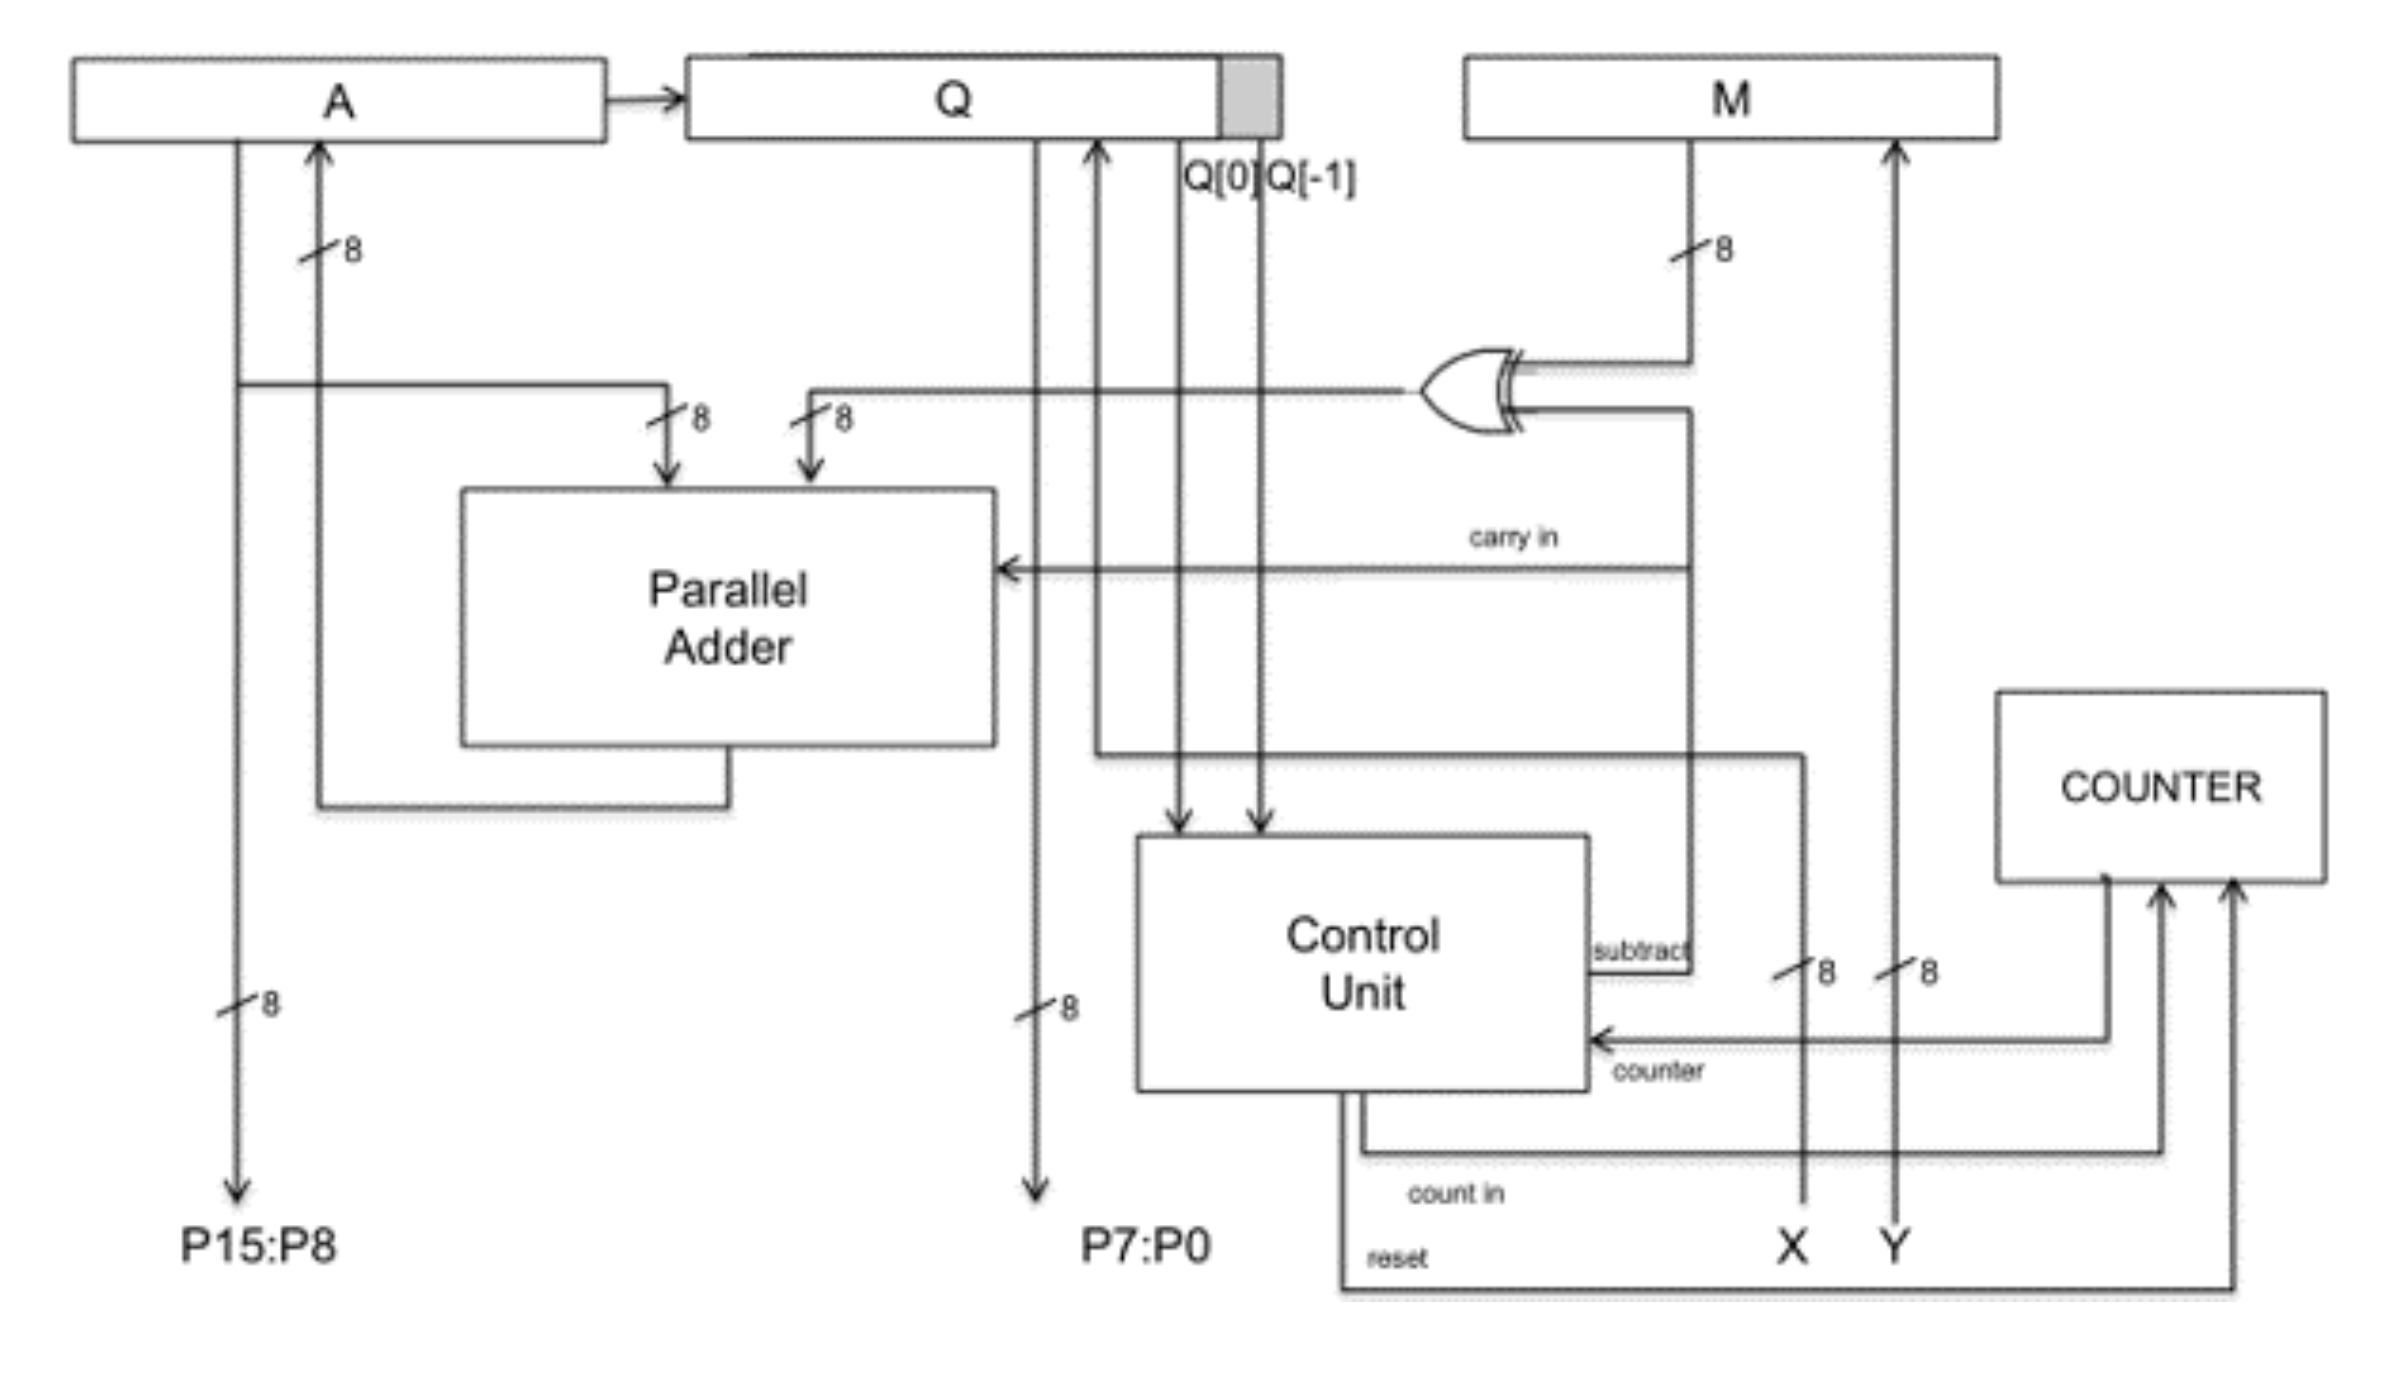
\includegraphics[width=1\textwidth]{img/Esercizio_7_1/booth_prog}
	\caption{Moltiplicatore di Booth}
	\label{booth_prog} 
\end{figure}

Le componenti necessarie sono quindi:
\begin{itemize}
    \item \textbf{Shift\_register}: uno per il valore $A$ (Accumulator), uno per il valore $Q$ e un terzo, il quale memorizzerà il il valore $M$ (quest'ultimo non avrà necessità di fare shift);
    \item \textbf{Flip-Flop D}: necessario per la memorizzazione del valore $Q_1$ e componente strutturale il contatore;
    \item \textbf{Counter}: contatore che porta il conteggio dei passi effettuati;
    \item \textbf{Parallel Adder}: un moltiplicatore parallelo per effettuare la somma: nell'esempio si utilizza un sommatore Carry-Look-Ahead;
    \item \textbf{Control unit}: unità di controllo per la gestione dell'unità operativa.
\end{itemize}

\subsubsection{Shift\_Register}
Lo Shift\_Register utilizzato differisce da quello visto in precedenza per la presenza di due ingressi aggiuntivi che consentono l'inizializzazione del registro e l'inserimento di un'intera stringa nel registro:

\begin{figure}[H]
	\centering
	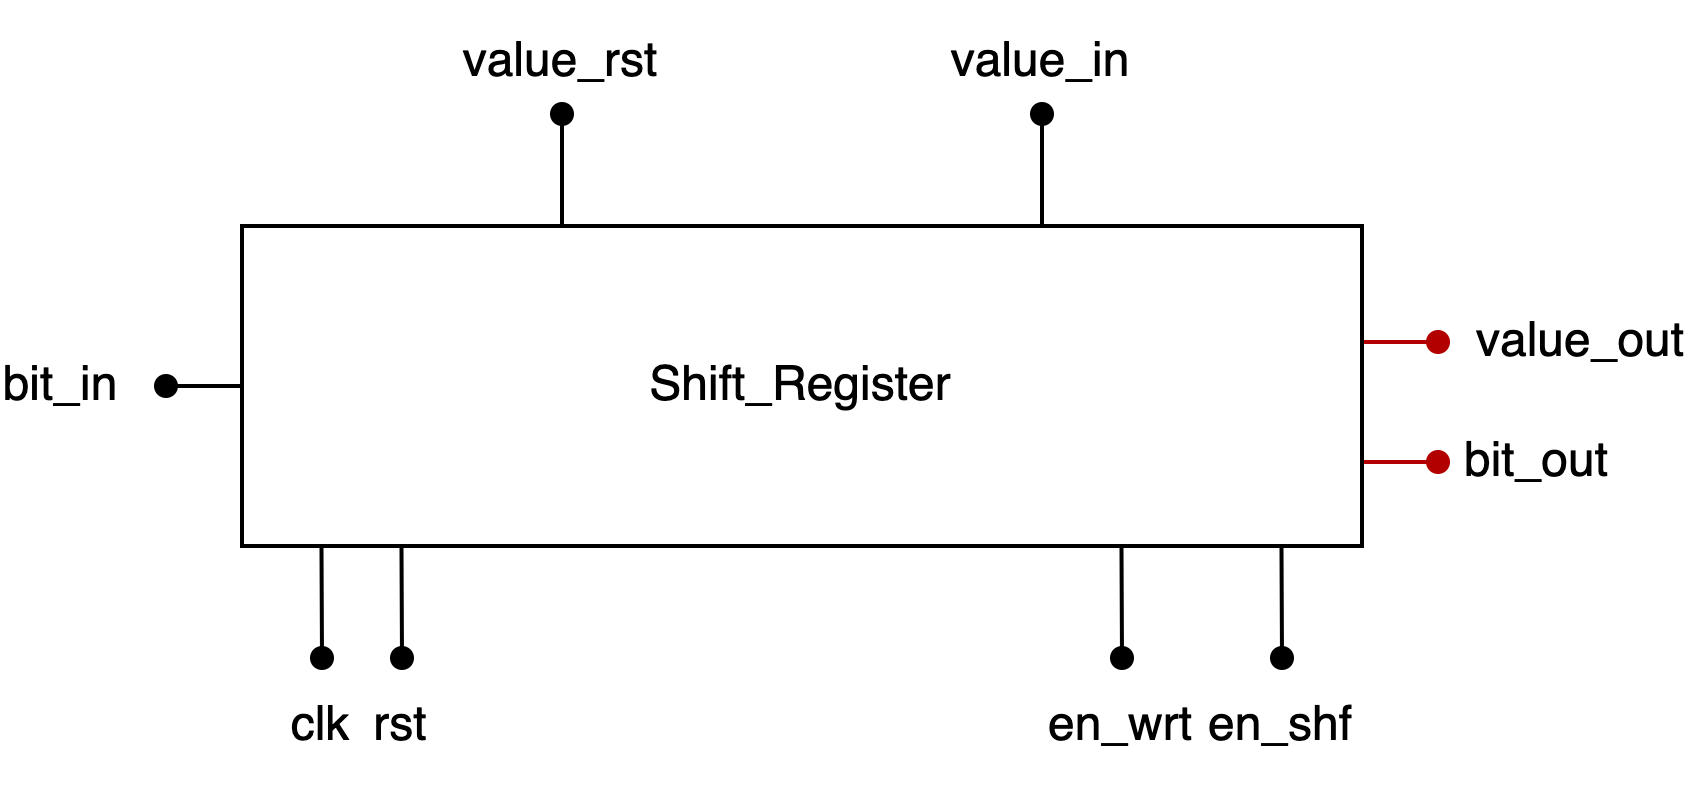
\includegraphics[width=1\textwidth]{img/Esercizio_7_1/Shift_Register_booth.png}
	\caption{Shift\_Register}
	\label{sh_booth} 
\end{figure}

\subsubsection{Flip-Flop D}
Il Flip-Flop D è lo stesso progettato nel capitolo (Citare capitolo).
Si deve notare, che alcune delle porte di ingresso del Flip-Flop D rimarranno inutilizzate, poiché in tale progetto non vi è la necessità di effettuare un settaggio iniziale.

\subsubsection{Counter}
La macchina counter è un contatore modulo 3.\\
Analogamente ai contatori presentati nell'esercizio del cronometro, esso si ottiene utilizzando 3 Flip-Flop D in parallelo.\\

\begin{figure}[H]
	\centering
	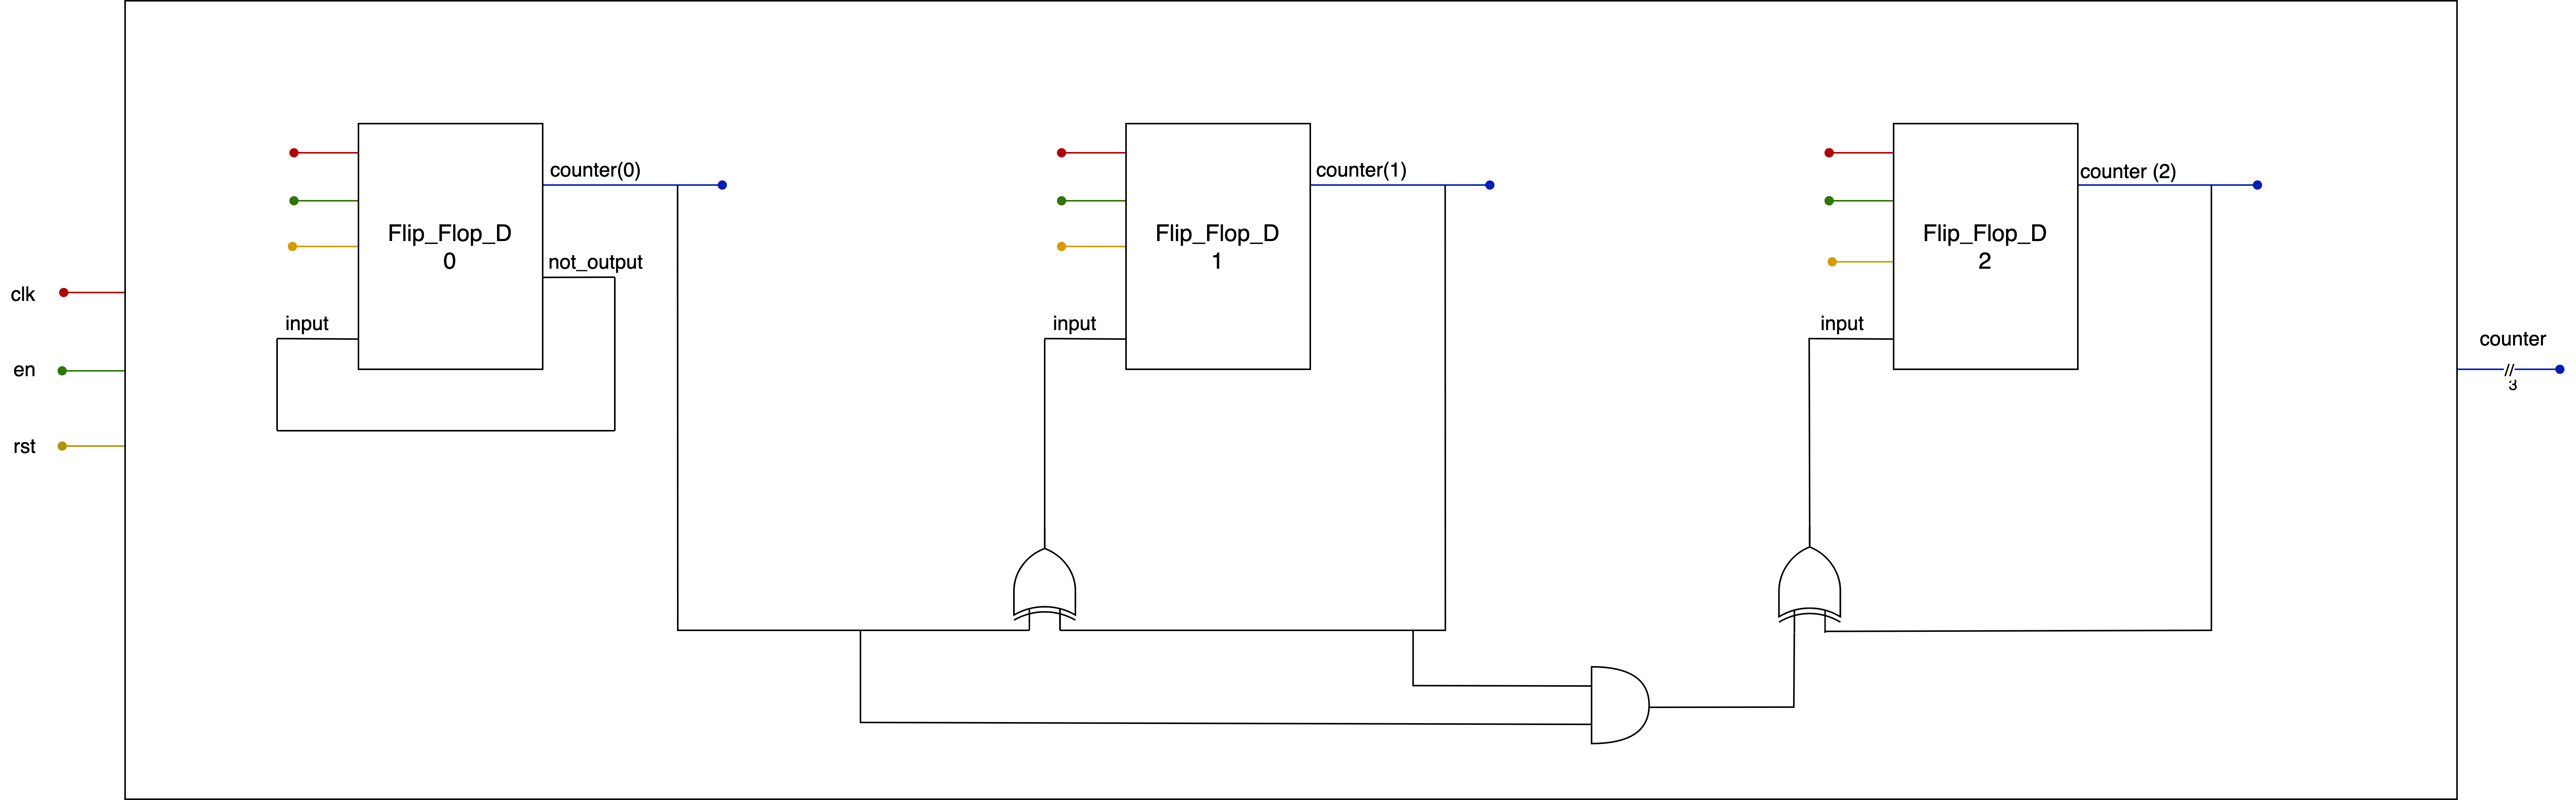
\includegraphics[width=1\textwidth]{img/Esercizio_7_1/counter_mod_8.png}
	\caption{Counter mod 8}
	\label{cnt_mod_8} 
\end{figure}

\subsubsection{Carry-Look-Ahead}
Per effettuare la somma, si necessita un sommatore parallelo.\\ 
Si vuole utilizzare il Carry-Look-Ahead (è possibile scegliere qualsiasi altro sommatore parallelo) con operandi ad 8 bits. 

\begin{figure}[H]
	\centering
	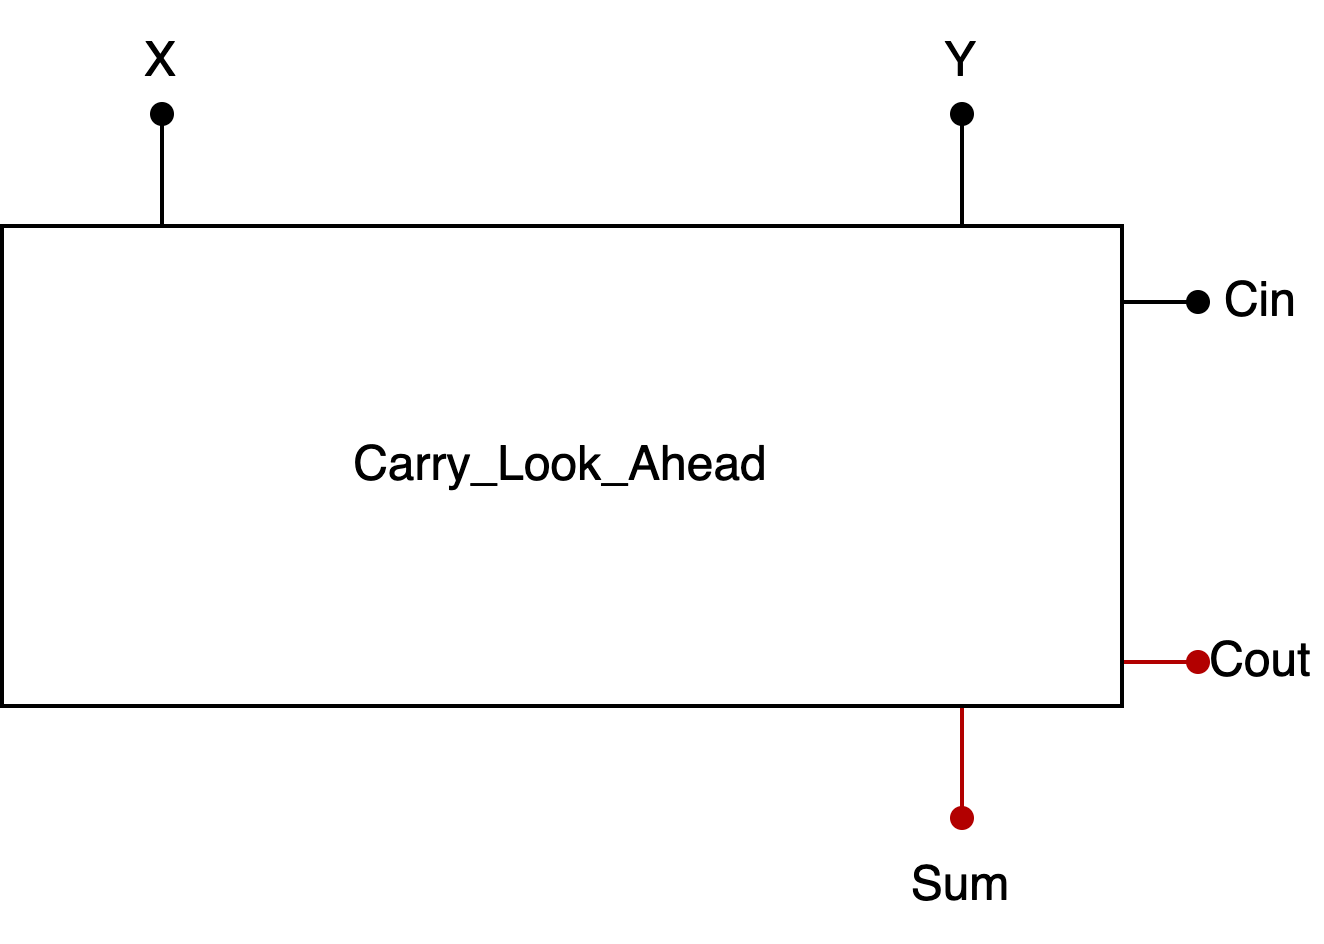
\includegraphics[width=0.7\textwidth]{img/Esercizio_7_1/carry_look_ahead_beh}
	\caption{Carry Look Ahead}
	\label{CLA} 
\end{figure}

Si noti che all'interno di tale sommatore, viene gestita la scelta di operare un'addizione o una sottrazione.

\subsubsection{Control Unit}
Per la gestione delle operazioni, si utilizza una Control Unit.\\
Essa altro non è che una macchina sequenziale e quindi va progettato l'automa a stati finiti corrispondente:

\begin{figure}[H]
	\centering
	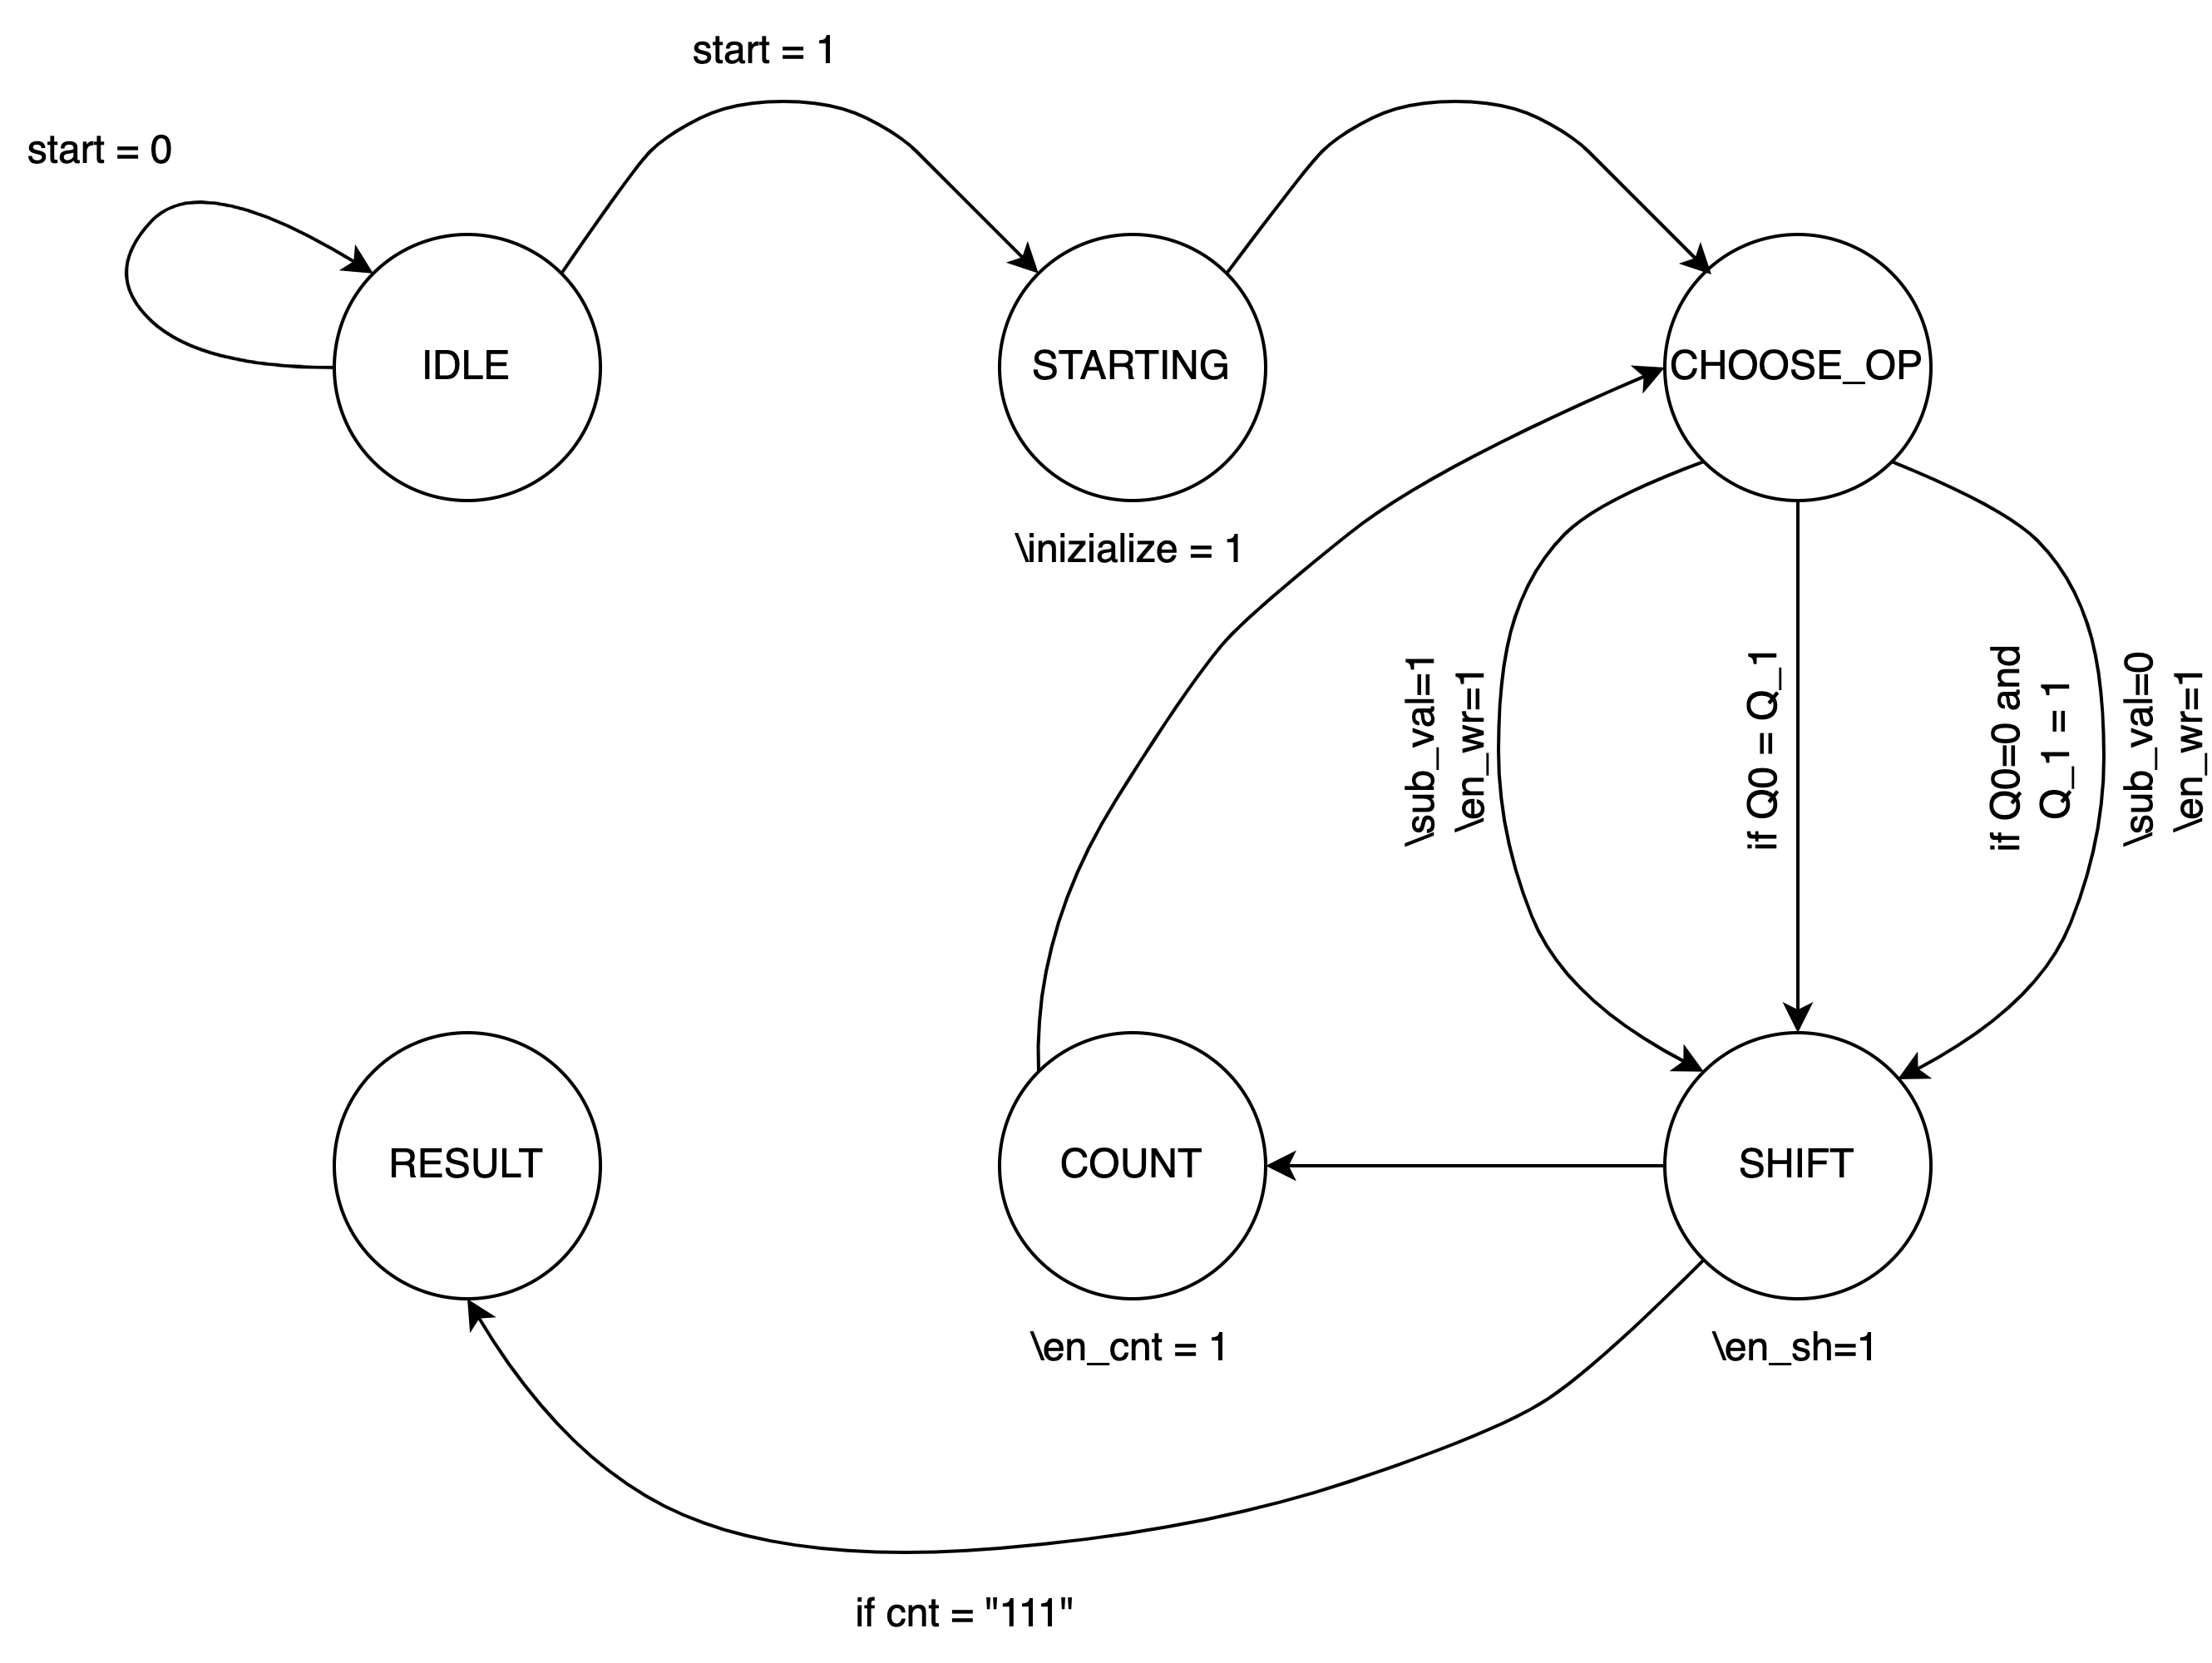
\includegraphics[width=1\textwidth]{img/Esercizio_7_1/booth_cu.png}
	\caption{Control Unit}
	\label{cu_automa} 
\end{figure}



\subsection{Implementazione}
\subsubsection{Shift\_Register}
L'implementazione dello Shift Register è la seguente:
 \begin{code}
    \inputminted[frame=lines, framesep=2mm, baselinestretch=1.2, bgcolor=LightGray, fontsize=\footnotesize, linenos]{vhdl}{vhdl_files/Esercizio_7_1/shift_register.vhdl}
    \caption{shift\_register.vhdl}
    \label{lbl:shr}
\end{code}

\subsubsection{Counter}
L'implementazione dello Counter è la seguente:
 \begin{code}
    \inputminted[frame=lines, framesep=2mm, baselinestretch=1.2, bgcolor=LightGray, fontsize=\footnotesize, linenos]{vhdl}{vhdl_files/Esercizio_7_1/counter_mod_8.vhdl}
    \caption{counter\_mod\_8.vhdl}
    \label{lbl:cnt_mod_8}
\end{code}

L'implementazione del Flip-Flop D è la stessa fatta in precedenza. %Citazione


\subsubsection{Carry-Look-Ahead}
L'implementazione del sommatore, con approccio comportamentale, è la seguente:
 \begin{code}
    \inputminted[frame=lines, framesep=2mm, baselinestretch=1.2, bgcolor=LightGray, fontsize=\footnotesize, linenos]{vhdl}{vhdl_files/Esercizio_7_1/carry_look_ahead.vhdl}
    \caption{carry\_look\_ahead.vhdl}
    \label{lbl:cla}
\end{code}

\subsubsection{Control Unit}
Lo sviluppo della Control Unit è esposto di seguito:
 \begin{code}
    \inputminted[frame=lines, framesep=2mm, baselinestretch=1.2, bgcolor=LightGray, fontsize=\footnotesize, linenos]{vhdl}{vhdl_files/Esercizio_7_1/cu.vhdl}
    \caption{cu.vhdl}
    \label{lbl:cu_booth}
\end{code}

\subsubsection{Booth}
Quindi a questo punto, si può implementare strutturalmente la macchina Booth:
 \begin{code}
    \inputminted[frame=lines, framesep=2mm, baselinestretch=1.2, bgcolor=LightGray, fontsize=\footnotesize, linenos]{vhdl}{vhdl_files/Esercizio_7_1/booth.vhdl}
    \caption{booth.vhdl}
    \label{lbl:booth}
\end{code}

\subsection{Simulazione}
Per effettuare la simulazione della macchina, è stato implementato il seguente test\_bench:
 \begin{code}
    \inputminted[frame=lines, framesep=2mm, baselinestretch=1.2, bgcolor=LightGray, fontsize=\footnotesize, linenos]{vhdl}{vhdl_files/Esercizio_7_1/booth_tb.vhdl}
    \caption{booth\_tb.vhdl}
    \label{lbl:tb_booth}
\end{code}

Il risultato è il seguente:

\begin{figure}[H]
	\centering
	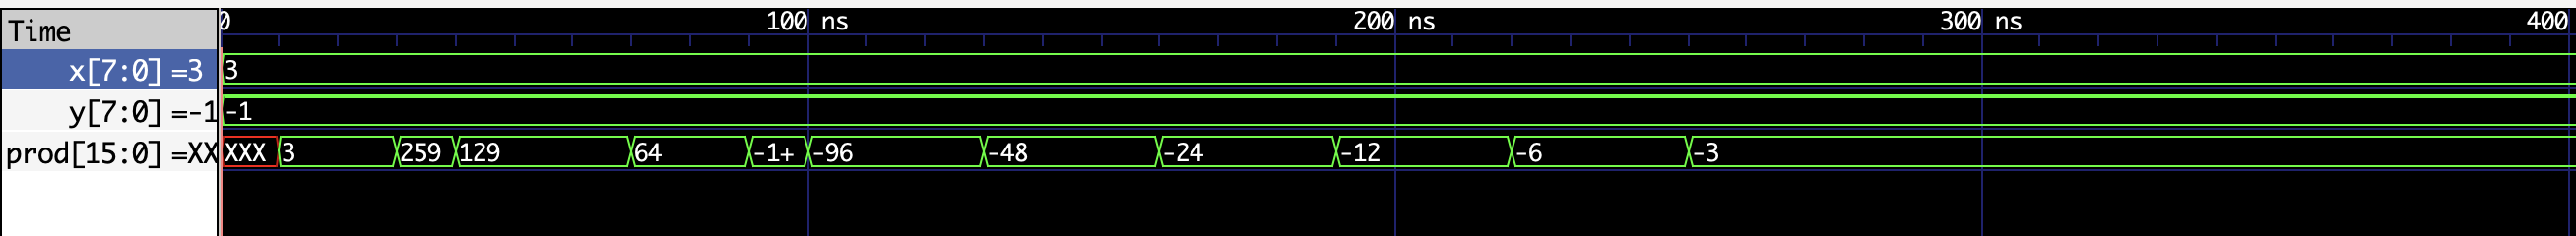
\includegraphics[width=1\textwidth]{img/Esercizio_7_1/booth_sim_1.png}
	\caption{Simulazione 1: $3 \times -1$}
	\label{booth_sim_1} 
\end{figure}

\begin{figure}[H]
	\centering
	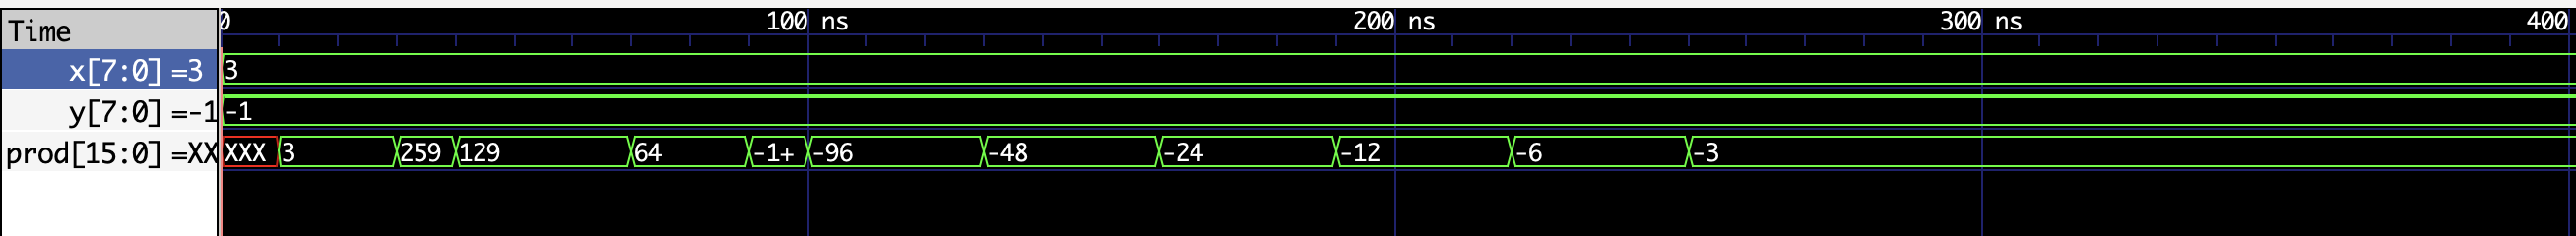
\includegraphics[width=1\textwidth]{img/Esercizio_7_1/booth_sim_1.png}
	\caption{Simulazione 1: $-13 \times -16$}
	\label{booth_sim_1} 
\end{figure}

\section{Implementazione su board del punto precedente}
\subsection{Traccia}
 Sintetizzare il moltiplicatore implementato al punto 7.1 su FPGA e testarlo mediante l’utilizzo dei dispositivi di input/output (switch, bottoni, led, display) presenti sulla board di sviluppo in dotazione. La modalità di utilizzo degli stessi è a completa discrezione degli 
studenti.
\subsection{Implementazione}
Per l'implementazione su board si è scelto di utilizzare gli switches da 0 a 7 per il primo operando e gli switches da 8 a 15 per il secondo operando. Per lo start si è utilizzato il bottone BTNU, mentre per il reset si è utilizzato il bottone centrale BTNC. Per realizzare ciò è stato utilizzato il seguente file \textit{Nexys-A7-50T-Master.xdc} come mostrato:
{\footnotesize
\begin{verbatim}
# Clock signal
set_property -dict { PACKAGE_PIN E3    IOSTANDARD LVCMOS33 } [get_ports { clk }]; 
#IO_L12P_T1_MRCC_35 Sch=clk100mhz
create_clock -add -name sys_clk_pin -period 100000 -waveform {0 5}
[get_ports {clk}];

##Switches
set_property -dict { PACKAGE_PIN J15   IOSTANDARD LVCMOS33 } 
[get_ports { X[0] }]; #IO_L24N_T3_RS0_15 Sch=sw[0]
set_property -dict { PACKAGE_PIN L16   IOSTANDARD LVCMOS33 } 
[get_ports { X[1]}]; #IO_L3N_T0_DQS_EMCCLK_14 Sch=sw[1]
set_property -dict { PACKAGE_PIN M13   IOSTANDARD LVCMOS33 } 
[get_ports { X[2] }]; #IO_L6N_T0_D08_VREF_14 Sch=sw[2]
set_property -dict { PACKAGE_PIN R15   IOSTANDARD LVCMOS33 } 
[get_ports { X[3] }]; #IO_L13N_T2_MRCC_14 Sch=sw[3]
set_property -dict { PACKAGE_PIN R17   IOSTANDARD LVCMOS33 } 
[get_ports { X[4] }]; #IO_L12N_T1_MRCC_14 Sch=sw[4]
set_property -dict { PACKAGE_PIN T18   IOSTANDARD LVCMOS33 } 
[get_ports { X[5] }]; #IO_L7N_T1_D10_14 Sch=sw[5]
set_property -dict { PACKAGE_PIN U18   IOSTANDARD LVCMOS33 } 
[get_ports { X[6] }]; #IO_L17N_T2_A13_D29_14 Sch=sw[6]
set_property -dict { PACKAGE_PIN R13   IOSTANDARD LVCMOS33 } 
[get_ports { X[7] }]; #IO_L5N_T0_D07_14 Sch=sw[7]
set_property -dict { PACKAGE_PIN T8    IOSTANDARD LVCMOS18 } 
[get_ports { Y[0] }]; #IO_L24N_T3_34 Sch=sw[8]
set_property -dict { PACKAGE_PIN U8    IOSTANDARD LVCMOS18 } 
[get_ports { Y[1] }]; #IO_25_34 Sch=sw[9]
set_property -dict { PACKAGE_PIN R16   IOSTANDARD LVCMOS33 } 
[get_ports { Y[2] }]; #IO_L15P_T2_DQS_RDWR_B_14 Sch=sw[10]
set_property -dict { PACKAGE_PIN T13   IOSTANDARD LVCMOS33 } 
[get_ports { Y[3] }]; #IO_L23P_T3_A03_D19_14 Sch=sw[11]
set_property -dict { PACKAGE_PIN H6    IOSTANDARD LVCMOS33 } 
[get_ports { Y[4] }]; #IO_L24P_T3_35 Sch=sw[12]
set_property -dict { PACKAGE_PIN U12   IOSTANDARD LVCMOS33 } 
[get_ports { Y[5] }]; #IO_L20P_T3_A08_D24_14 Sch=sw[13]
set_property -dict { PACKAGE_PIN U11   IOSTANDARD LVCMOS33 } 
[get_ports { Y[6] }]; #IO_L19N_T3_A09_D25_VREF_14 Sch=sw[14]
set_property -dict { PACKAGE_PIN V10   IOSTANDARD LVCMOS33 } 
[get_ports { Y[7] }]; #IO_L21P_T3_DQS_14 Sch=sw[15]

## LEDs
set_property -dict { PACKAGE_PIN H17   IOSTANDARD LVCMOS33 } 
[get_ports { res[0] }]; #IO_L18P_T2_A24_15 Sch=led[0]
set_property -dict { PACKAGE_PIN K15   IOSTANDARD LVCMOS33 } 
[get_ports { res[1] }]; #IO_L24P_T3_RS1_15 Sch=led[1]
set_property -dict { PACKAGE_PIN J13   IOSTANDARD LVCMOS33 } 
[get_ports { res[2] }]; #IO_L17N_T2_A25_15 Sch=led[2]
set_property -dict { PACKAGE_PIN N14   IOSTANDARD LVCMOS33 } 
[get_ports { res[3] }]; #IO_L8P_T1_D11_14 Sch=led[3]
set_property -dict { PACKAGE_PIN R18   IOSTANDARD LVCMOS33 } 
[get_ports { res[4] }]; #IO_L7P_T1_D09_14 Sch=led[4]
set_property -dict { PACKAGE_PIN V17   IOSTANDARD LVCMOS33 } 
[get_ports { res[5] }]; #IO_L18N_T2_A11_D27_14 Sch=led[5]
set_property -dict { PACKAGE_PIN U17   IOSTANDARD LVCMOS33 } 
[get_ports { res[6] }]; #IO_L17P_T2_A14_D30_14 Sch=led[6]
set_property -dict { PACKAGE_PIN U16   IOSTANDARD LVCMOS33 } 
[get_ports { res[7] }]; #IO_L18P_T2_A12_D28_14 Sch=led[7]
set_property -dict { PACKAGE_PIN V16   IOSTANDARD LVCMOS33 } 
[get_ports { res[8] }]; #IO_L16N_T2_A15_D31_14 Sch=led[8]
set_property -dict { PACKAGE_PIN T15   IOSTANDARD LVCMOS33 } 
[get_ports { res[9] }]; #IO_L14N_T2_SRCC_14 Sch=led[9]
set_property -dict { PACKAGE_PIN U14   IOSTANDARD LVCMOS33 } 
[get_ports { res[10] }]; #IO_L22P_T3_A05_D21_14 Sch=led[10]
set_property -dict { PACKAGE_PIN T16   IOSTANDARD LVCMOS33 } 
[get_ports { res[11] }]; #IO_L15N_T2_DQS_DOUT_CSO_B_14 Sch=led[11]
set_property -dict { PACKAGE_PIN V15   IOSTANDARD LVCMOS33 } 
[get_ports { res[12] }]; #IO_L16P_T2_CSI_B_14 Sch=led[12]
set_property -dict { PACKAGE_PIN V14   IOSTANDARD LVCMOS33 } 
[get_ports { res[13] }]; #IO_L22N_T3_A04_D20_14 Sch=led[13]
set_property -dict { PACKAGE_PIN V12   IOSTANDARD LVCMOS33 } 
[get_ports { res[14] }]; #IO_L20N_T3_A07_D23_14 Sch=led[14]
set_property -dict { PACKAGE_PIN V11   IOSTANDARD LVCMOS33 } 
[get_ports { res[15] }]; #IO_L21N_T3_DQS_A06_D22_14 Sch=led[15]

##Buttons
#set_property -dict { PACKAGE_PIN C12   IOSTANDARD LVCMOS33 } 
[get_ports { reset }]; #IO_L3P_T0_DQS_AD1P_15 Sch=cpu_resetn
set_property -dict { PACKAGE_PIN N17   IOSTANDARD LVCMOS33 } 
[get_ports { rst }]; #IO_L9P_T1_DQS_14 Sch=btnc
set_property -dict { PACKAGE_PIN M18   IOSTANDARD LVCMOS33 } 
[get_ports { start }]; #IO_L4N_T0_D05_14 Sch=btnu
#set_property -dict { PACKAGE_PIN P17   IOSTANDARD LVCMOS33 } 
[get_ports { load_i }]; #IO_L12P_T1_MRCC_14 Sch=btnl
#set_property -dict { PACKAGE_PIN M17   IOSTANDARD LVCMOS33 } 
[get_ports { load_M }]; #IO_L10N_T1_D15_14 Sch=btnr
#set_property -dict { PACKAGE_PIN P18   IOSTANDARD LVCMOS33 } 
[get_ports { BTND }]; #IO_L9N_T1_DQS_D13_14 Sch=btnd

\end{verbatim}
}
Da cui si osserva come sono state collegate le componenti utilizzate.\\
In seguito si mostrano alcune immagini del funzionamento del moltiplicatore sulla board.
\begin{figure}[H]
	\centering
	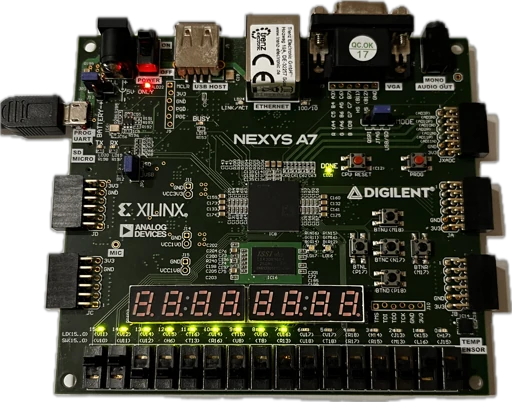
\includegraphics[width=0.8\textwidth]{img/onBoard/booth_test1}
	\caption{Test 1}
	\label{test1} 
\end{figure}
Nell'immagine rappresentante il Test 1 si è svolta la seguente moltiplicazione:\\
$11000000 * 00000010 = 1111111110000000$\\
che convertita in decimale risulta\\
$-64 * 2 = -128$\\
avendo utilizzato la notazione in complemento a 2.
\begin{figure}[H]
	\centering
	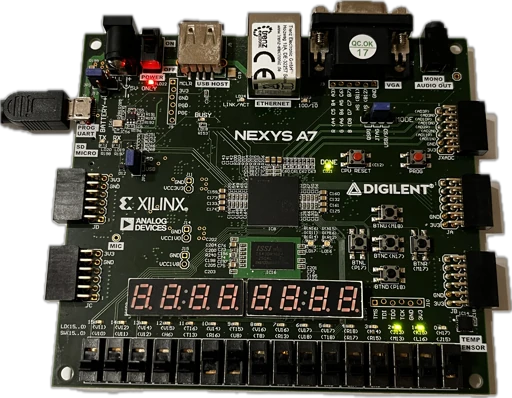
\includegraphics[width=0.8\textwidth]{img/onBoard/booth_test2}
	\caption{Test 2}
	\label{test1} 
\end{figure}
In Test 2 invece si è svolta la seguente moltiplicazione\\
$00000110 * 00000001 = 0000000000000110$ \\
che convertita in decimale risulta\\
$3 * 1 = 3$\\.
